\documentclass[12pt,letterpaper]{article}
% Paquetes del preambulo original, corregidos y ampliados
\usepackage[utf8]{inputenc}
\usepackage[T1]{fontenc}
\usepackage[spanish,es-tabla]{babel}
\usepackage{lmodern}
\usepackage{amsmath,amsfonts,amssymb}
\usepackage{graphicx}
\usepackage{geometry}
\usepackage{fancyhdr}
\usepackage{listings}
\usepackage{xcolor}
\usepackage{float}
\usepackage{hyperref}
\usepackage{longtable,booktabs,array}
\usepackage{calc}
\usepackage{enumitem}
\usepackage{microtype}
\usepackage{xltabular}
\usepackage{array}
\usepackage{booktabs}
\usepackage[backend=biber,style=ieee]{biblatex}
\addbibresource{referencias.bib}
\geometry{top=2.5cm,bottom=2.5cm,left=2.5cm,right=2.5cm}
\setlength{\parindent}{0pt}
\setlength{\parskip}{5pt}
\renewcommand{\baselinestretch}{1.28}
\setlength{\headheight}{16pt}
\pagestyle{fancy}
\fancyhf{}
\fancyhead[L]{CE1108 -- Compiladores e Intérpretes}
\fancyhead[R]{Proyecto 1}
\fancyfoot[C]{\thepage}
\hypersetup{colorlinks=true,linkcolor=blue!45!black,urlcolor=blue!45!black,citecolor=blue!45!black,pdftitle={Documentacion general BALC},pdfauthor={Equipo BALC}}
\definecolor{codigoFondo}{RGB}{248,249,251}
\definecolor{codigoBorde}{RGB}{187,193,200}
\lstdefinestyle{codigoBALC}{
 basicstyle=\ttfamily\scriptsize,
 keywordstyle=\color{blue!60!black}\bfseries,
 stringstyle=\color{red!55!black},
 commentstyle=\color{green!40!black}\itshape,
 numbers=left,numberstyle=\tiny\color{gray},numbersep=7pt,
 frame=single,rulecolor=\color{codigoBorde},backgroundcolor=\color{codigoFondo},
 breaklines=true,breakatwhitespace=false,showstringspaces=false,
 tabsize=4,captionpos=b,columns=fullflexible,keepspaces=true
}
\lstset{style=codigoBALC}
\providecommand{\tightlist}{\setlength{\itemsep}{0pt}\setlength{\parskip}{0pt}}
\providecommand{\passthrough}[1]{#1}
\providecommand{\pandocbounded}[1]{#1}
\setcounter{tocdepth}{2}
\begin{document}
\begin{titlepage}
\centering
{\Large Instituto Tecnológico de Costa Rica\par}
\vspace{0.25cm}
{\large Escuela de Ingeniería en Computadores\par}
\vfill
%\IfFileExists{fig_logo.png}{\includegraphics[width=0.55\textwidth]{fig_logo.png}}{\fbox{\parbox[c][2.6cm][c]{0.52\textwidth}{\centering Logotipo institucional\\[3pt]\footnotesize Agregar \\texttt{fig\_logo.png}}}}
\vfill
{\bfseries\LARGE Compiladores e Intérpretes\par}
\vspace{0.45cm}
{\bfseries\Large Proyecto I - Compilador para código binario \par}
\vspace{0.2cm}
{\large Compilador para una arquitectura VLIW\par}
\vfill
\begin{flushleft}
\textbf{Integrantes:}\\[0.20cm]
\begin{tabular}{@{}p{0.69\textwidth}l@{}}
Meibel Elena Mora Brenes & 2021128644\\
Dylan Maximiliano Guerrero Gonzaléz & 2022016016\\
José García Izaguirre & 2022437991\\
Javier Hernández Castillo & 2022321746\\
\end{tabular}\\[0.45cm]
\textbf{Profesor:} Jason Leitón Jiménez\\[0.15cm]
\textbf{Grupo:} 1\\[0.15cm]
\textbf{Semestre:} II Semestre 2026
\end{flushleft}
\vfill
\end{titlepage}
\tableofcontents
\clearpage
\section{Resumen ejecutivo}\label{1-resumen-ejecutivo}

BALC es un compilador escrito en C que recibe un archivo fuente en el
lenguaje BAL y produce instrucciones para una microarquitectura VLIW específica.
Integra reconocimiento de tokens, análisis sintáctico con AST, análisis
semántico con ámbitos, cálculo de ubicaciones de memoria, generación de
ensamblador, enlace y resolución de saltos, y codificación binaria. Los
formatos de salida son \texttt{.asm} (representación
textual por bundles), \texttt{.bin}(contenedor BALB
v1) y \texttt{.mem} (hexadecimal para memoria de
instrucciones).


\section{Arquitectura del compilador y
herramientas}\label{2-arquitectura-del-compilador-y-herramientas}

\subsection{Fases}\label{21-fases}

\begin{lstlisting}
archivo .bal
    |
    v
Lexer (Flex) -> secuencia de tokens
    |
    v
Parser (Bison) -> AST
    |
    v
Analisis semantico -> tabla de simbolos y ambitos
    |
    v
Asignacion de memoria -> globales, pila y marcos
    |
    v
Generacion de instrucciones -> ensamblador interno
    |
    v
Enlace de funciones y resolucion de referencias
    |
    v
Layout VLIW y expansion de saltos lejanos
    |
    v
Codificacion -> .asm, .bin BALB v1 y .mem
\end{lstlisting}
\newpage
\subsection{Organización del
repositorio}\label{22-organizaciuxf3n-del-repositorio}

\begin{xltabular}{\textwidth}{@{}p{0.22\textwidth}p{0.4\textwidth}X@{}}
\toprule\noalign{}
Área & Archivos relevantes & Función \\
\midrule\noalign{}
\endhead
\bottomrule\noalign{}
\endlastfoot
Entrada / CLI & \path{src/main.c},
\path{src/cli.c},
\path{include/cli.h} & Opciones y orquestación. \\
Lexer & \path{src/lexer.l},
\path{src/lexer.c},
\path{src/token.c} & Tokens, ubicaciones y
diagnóstico léxico. \\
Parser y AST &
\path{Analisis_Sintactico/gramatica.y},
\path{ast.c},
\path{puente/lexer.c} & Gramática, construcción del
árbol y enlace con el lexer. \\
Símbolos y semántica &
\path{Analisis_Semantico/symbol_table.c},
\path{semantic.c},
\path{semantic_modules.c} & Tipos, ámbitos,
funciones y módulos. \\
Memoria & \path{Analisis_Semantico/memory.c} &
Almacenes, offsets y marcos de pila. \\
Backend & \path{src/generacion_basica.c},
\path{generacion_control.c},
\path{generacion_funciones.c},
\path{generacion_adaptador.c} & Emisión de código
para expresiones, control y funciones. \\
Referencias y enlace &
\path{src/resolucion_referencias.c},
\path{referencias_integracion.c},
\path{resolucion_saltos.c},
\path{enlace_funciones.c} & Direcciones y saltos. \\
Binario & \path{src/codificacion_binaria.c},
\path{formato_binario.c} & Verificación y escritura
de \path{.bin} y \path{.mem}. \\
Pruebas & \texttt{tests/} & Verificaciones de etapas y
de programas ejemplo. \\
\end{xltabular}

\textbf{Requisitos de construcción informados por el repositorio:}
compilador GCC con C11, GNU Make, Flex y Bison. En Ubuntu:
\texttt{sudo apt install build-essential flex bison};
luego \texttt{make} y
\texttt{make test}.
\newpage
\subsection{Interfaz de línea de
comandos}\label{23-interfaz-de-luxednea-de-comandos}

\begin{lstlisting}[language=bash]
./balc [-o archivo.bin] [-v] [-s] [-t] [-m] [-p] programa.bal
./balc -x [-o archivo.bin] [-v] [-p] programa.asm
\end{lstlisting}

\begin{longtable}[]{@{}p{0.280\linewidth}p{0.660\linewidth}@{}}
\toprule\noalign{}
Opción & Efecto \\
\midrule\noalign{}
\endhead
\bottomrule\noalign{}
\endlastfoot
\texttt{-o archivo} & Define nombre de salida del
archivo binario. \\
\texttt{-v} & Informa las etapas de compilación. \\
\texttt{-s} & Emite también ensamblador
\texttt{.asm}. \\
\texttt{-t} & Muestra el AST. \\
\texttt{-m} & Muestra símbolos y asignación de
memoria. \\
\texttt{-p} & Imprime bundles, direcciones y
codificación. \\
\texttt{-x} & Codifica un archivo
\texttt{.asm} directamente. \\
\texttt{--frontend} & Analiza entrada sin ejecutar el
backend. \\
\end{longtable}

No debe confundirse la generación de archivos con su ejecución en el
procesador.

\section{Especificación de la arquitectura destino}\label{3-especificaciuxf3n-de-la-arquitectura-destino--apartado-81}

El contrato proviene de la ISA del proyecto del curso Arquitectura de
Computadores I. El tamaño de instrucción es \textbf{32 bits} y cada
bundle VLIW contiene \textbf{4 slots de 32 bits}, total \textbf{128 bits
= 16 bytes}, asociados a \textbf{ALU, LSU, BRU y CRIPTO}. El PC de
instrucciones se expresa en bytes y las direcciones de bundles están
alineadas a 16 bytes. Memoria de \textbf{64 KiB}, direccionada por bytes
y little-endian. Registros generales: \textbf{32 de 32 bits}. Los
inmediatos y desplazamientos con signo se interpretan en complemento a
dos, según el campo correspondiente.

\subsection{Green card de la ISA del proyecto
VLIW}\label{green-card-de-la-isa-del-proyecto-vliw}

Todas las instrucciones miden 32 bits: \textbf{Tipo de operación}
{[}31:25{]} (7 bits) + \textbf{ID de operación} {[}24:21{]} (4 bits) +
operandos (21 bits, según el tipo). Los campos de registro usan 5 bits
(x0--x31).
\newpage
\subsubsection{Instrucciones tipo
almacenar}\label{instrucciones-tipo-almacenar}

\begin{longtable}[]{@{}p{0.15\linewidth}p{0.240\linewidth}p{0.6\linewidth}@{}}
\toprule\noalign{}
Mnemónico & Nombre & Descripción / ejemplo \\
\midrule\noalign{}
\endhead
\bottomrule\noalign{}
\endlastfoot
\texttt{guardap} & Guardar palabra &
\texttt{M(rf1+offset) = rf2[31:0]}. Ej.:
\texttt{guardap x3, x8, 5} $\rightarrow$ si x3 = 0x20, guarda en
0x25 el contenido de x8 \\
\texttt{guardab} & Guardar byte &
\texttt{M(rf1+offset) = rf2[7:0]}. Igual que
\texttt{guardap} pero solo guarda el byte menos
significativo. \\
\texttt{cargai} & Cargar palabra &
\texttt{rg = M[rf1 + offset]}, con
\texttt{rg} en {[}15:11{]}. Ej.: rf1 = 1000, offset =
20 $\rightarrow$ rg = M{[}1020{]}. \\
\texttt{cargabai} & Cargar byte &
\texttt{rg = signo(M8[rf1 + offset])}, con
\texttt{rg} en {[}15:11{]}; el byte se extiende con
signo. Ej.: rf1 = 2000, offset = 4, M8{[}2004{]} = 0x7F $\rightarrow$ rg =
0x0000007F; si fuera 0xFF $\rightarrow$ rg = 0xFFFFFFFF. \\
\end{longtable}

\subsubsection{Instrucciones tipo
inmediato}\label{instrucciones-tipo-inmediato}

\begin{xltabular}{\textwidth}{@{}Xp{0.33\textwidth}p{0.5\textwidth}@{}}
\toprule\noalign{}
Mnemónico & Nombre & Descripción / ejemplo \\
\midrule\noalign{}
\endhead
\bottomrule\noalign{}
\endlastfoot
\texttt{sumai} & Suma con inmediato &
\texttt{rg = rf1 + inm}. Ej.: rf1 = 10, inm = 5 $\rightarrow$ rg =
15. \\
\texttt{restai} & Resta con inmediato &
\texttt{rg = rf1 - inm}. Ej.: rf1 = 10, inm = 3 $\rightarrow$ rg =
7. \\
\texttt{cizqi} & Corrimiento izquierdo inmediato &
\texttt{rg = rf1 \textless{}\textless{} inm}. Ej.: \texttt{00000101 \textless{}\textless{} 2 = 00010100} (20). \\
\texttt{cderi} & Corrimiento derecho lógico inmediato &
\texttt{rg = rf1 \textgreater{}\textgreater{} inm}, rellena con ceros. Ej.:
\texttt{00010100 \textgreater{}\textgreater{} 2 = 00000101} (5). \\
\texttt{caderi} & Corrimiento aritmético derecho
inmediato & \texttt{rg = rf1 \textgreater{}\textgreater{}\textgreater{} inm}, conserva el
signo. Ej.: \texttt{11110000 \textgreater{}\textgreater{}\textgreater{} 2 = 11111100}. \\
\texttt{xori} & XOR con inmediato &
\texttt{rg = rf1 XOR inm}. Ej.:
\texttt{1010 XOR 1100 = 0110}. \\
\texttt{andi} & AND con inmediato &
\texttt{rg = rf1 AND inm}. Ej.:
\texttt{1010 AND 1100 = 1000}. \\
\texttt{ori} & OR con inmediato &
\texttt{rg = rf1 OR inm}. Ej.:
\texttt{1010 OR 1100 = 1110}. \\
\end{xltabular}

\subsubsection{Instrucciones tipo salto}\label{instrucciones-tipo-salto}

\begin{xltabular}{\textwidth}{@{}Xp{0.25\textwidth}p{0.6\textwidth}@{}}
\toprule\noalign{}
Mnemónico & Nombre & Descripción / ejemplo \\
\midrule\noalign{}
\endhead
\bottomrule\noalign{}
\endlastfoot
\texttt{sye} & Saltar y enlazar &
\texttt{rg = PC + 16; PC = PC + offset} (offset de 16
bits con signo, en bytes desde el PC del bundle y múltiplo de 16). Ej.:
PC = 1024, offset = 64 $\rightarrow$ rg = 1040, PC = 1088. \\
\texttt{syer} & Saltar y enlazar con registro &
\texttt{rg = PC + 16; PC = (rf1 + offset) AND 0xFFFFFFF0}
(offset de 11 bits con signo, en bytes). Ej.:
\texttt{syer x0, ra, 0} vuelve de una subrutina. \\
\end{xltabular}

\subsubsection{Instrucciones tipo
control}\label{instrucciones-tipo-control}

\begin{longtable}[]{@{}p{0.15\linewidth}p{0.240\linewidth}p{0.6\linewidth}@{}}
\toprule\noalign{}
Mnemónico & Nombre & Descripción / ejemplo \\
\midrule\noalign{}
\endhead
\bottomrule\noalign{}
\endlastfoot
\texttt{igualsi} & Saltar si igual &
\texttt{if (rf1 == rf2) PC += inm} (inm en bytes,
múltiplo de 16). Ej.:
\texttt{igualsi rf1=3, rf2=4, inmediato=64} salta 4
bundles. \\
\texttt{igualno} & Saltar si no es igual &
{\lstinline"if (rf1 != rf2) PC += inm"}. Ej.:
\texttt{igualno rf1=5, rf2=6, inmediato=96} salta 6
bundles. \\
\texttt{menora} & Saltar si menor &
\texttt{if (rf1 \textless{} rf2) PC += inm}, con signo. Ej.:
\texttt{menora rf1=7, rf2=8, inmediato=48} salta 3
bundles. \\
\texttt{mayoroigual} & Saltar si mayor o igual &
\texttt{if (rf1 \textgreater{}= rf2) PC += inm}, con signo. Ej.:
\texttt{mayoroigual rf1=9, rf2=10, inmediato=80} salta
5 bundles. \\
\end{longtable}

\subsubsection{Instrucciones tipo
registro}\label{instrucciones-tipo-registro}

\begin{longtable}[]{@{}p{0.15\linewidth}p{0.240\linewidth}p{0.6\linewidth}@{}}
\toprule\noalign{}
Mnemónico & Nombre & Descripción / ejemplo \\
\midrule\noalign{}
\endhead
\bottomrule\noalign{}
\endlastfoot
\texttt{suma} & Suma &
\texttt{rg = rf1 + rf2}. \\
\texttt{resta} & Resta &
\texttt{rg = rf1 - rf2}. \\
\texttt{cizq} & Corrimiento izquierdo &
\texttt{rg = rf1 \textless{}\textless{} rf2}. Ej.: rf1 = 5, rf2 = 2 $\rightarrow$ rg =
20. \\
\texttt{cder} & Corrimiento derecho lógico &
\texttt{rg = rf1 \textgreater{}\textgreater{} rf2}, rellena con ceros. Ej.: rf1 =
20, rf2 = 2 $\rightarrow$ rg = 5. \\
\texttt{cader} & Corrimiento aritmético derecho &
\texttt{rg = rf1 \textgreater{}\textgreater{}\textgreater{} rf2}, conserva el signo. Ej.: rf1
= -8, rf2 = 2 $\rightarrow$ rg = -2. \\
\texttt{xor} & XOR &
\texttt{rg = rf1 XOR rf2}. Ej.:
\texttt{1010 XOR 1100 = 0110}. \\
\texttt{and} & AND &
\texttt{rg = rf1 AND rf2}. Ej.:
\texttt{1010 AND 1100 = 1000} (8). \\
\texttt{or} & OR &
\texttt{rg = rf1 OR rf2}. Ej.:
\texttt{1010 OR 1100 = 1110} (14). \\
\texttt{mrq} & Menor que &
\texttt{rg = (rf1 \textless{} rf2) ? 1 : 0}. Ej.: rf1 = 5, rf2 =
10 $\rightarrow$ rg = 1. \\
\texttt{myq} & Mayor que &
\texttt{rg = (rf1 \textgreater{} rf2) ? 1 : 0}. Ej.: rf1 = 10, rf2 =
5 $\rightarrow$ rg = 1. \\
\end{longtable}
\subsubsection{Instrucciones tipo cripto}\label{instrucciones-tipo-cripto}

\begin{xltabular}{\textwidth}{@{}Xp{0.25\textwidth}p{0.6\textwidth}@{}}
\toprule\noalign{}
Mnemónico & Nombre & Descripción / ejemplo \\
\midrule\noalign{}
\endhead
\bottomrule\noalign{}
\endlastfoot
\texttt{fsl} & Ronda Feistel &
\texttt{(L\_out, R\_out) = (R, L XOR F(R, K))} con
\texttt{K = boveda[LK][RK]}; lee el par (r1, r1+1) y
escribe (rd, rd+1). Cifrar = 4 \texttt{fsl} con RK =
0..3. Ej.: \texttt{fsl rd=6, r1=2, LK=0, RK=1}. \\
\texttt{fsli} & Ronda Feistel inversa &
\texttt{(L\_out, R\_out) = (R XOR F(L, K), L)}: deshace
una \texttt{fsl}. Descifrar = 4
\texttt{fsli} con RK = 3..0. Ej.:
\texttt{fsli rd=6, r1=2, LK=0, RK=3}. \\
\texttt{ell} & Escribir llave en la bóveda &
\texttt{boveda[LK][off..off+1] = (rs1, rs2)}, escribe
64 bits. Ej.: \texttt{ell LK=2, off=0, rs1=4, rs2=6} y
\texttt{ell LK=2, off=2, rs1=8, rs2=10} cargan la llave
completa. \\
\texttt{vcr} & Validar credenciales &
\texttt{AUTH = (M[dir\_cand] == contrasena de la boveda)};
el resultado sólo queda en ESTADO. Ej.:
\texttt{vcr dir\_cand=0x2000}. \\
\texttt{camcon} & Cambiar contraseña &
\texttt{contrasena = ROL(contrasena, imm)} y
\texttt{M[dir] = ROL(M[dir], imm)}; requiere
\texttt{AUTH = 1}. Ej.:
\texttt{camcon dir=0x0010, imm=7}. \\
\texttt{setpwd} & Inicializar contraseña &
\texttt{contrasena de la boveda = rs}; sólo con
\texttt{INIT = 1}, y después
\texttt{INIT = 0}. Ej.:
\texttt{setpwd rs=5}. \\
\end{xltabular}

\subsubsection{Pseudoinstrucciones}\label{pseudoinstrucciones}

\begin{longtable}[]{@{}p{0.190\linewidth}p{0.240\linewidth}p{0.510\linewidth}@{}}
\toprule\noalign{}
Mnemónico & Nombre & Descripción / ejemplo \\
\midrule\noalign{}
\endhead
\bottomrule\noalign{}
\endlastfoot
\texttt{nop} & No operación & Se codifica como
\texttt{0x00000000}. \\
\texttt{mov} & Mover &
\texttt{mov rg, rf1} $\rightarrow$
\texttt{suma rg, rf1, x0}. \\
\texttt{not} & Negación bit a bit &
\texttt{not rg, rf1} $\rightarrow$
\texttt{xori rg, rf1, -1}. \\
\texttt{ret} & Retornar & \texttt{ret}
$\rightarrow$ \texttt{syer x0, ra, 0}. \\
\end{longtable}

\subsubsection{Codificación por tipo}\label{codificaciuxf3n-por-tipo}

\begin{xltabular}{\textwidth}{
    @{}
    >{\hsize=0.5\hsize\linewidth=\hsize\raggedright\arraybackslash}X
    >{\hsize=0.5\hsize\linewidth=\hsize\raggedright\arraybackslash}X
    >{\hsize=1.5\hsize\linewidth=\hsize\raggedright\arraybackslash}X
    >{\hsize=0.5\hsize\linewidth=\hsize\raggedright\arraybackslash}X
    @{}
}
\toprule
Tipo de instrucción & Tipo (7 bits) & Formato & IDs \\
\midrule
\endhead

\bottomrule
\endlastfoot

Almacenar &
\texttt{1001001} &
Tipo \textbar{} ID \textbar{}
rf1 [20:16] \textbar{}
rf2 / rg [15:11] \textbar{}
offset [10:0] &
guardap 0000\newline guardab 0001\newline
cargai 1000\newline cargabai 1001 \\

\addlinespace

Inmediato &
\texttt{1000000} &
Tipo \textbar{} ID \textbar{}
rf1 [20:16] \textbar{}
rg [15:11] \textbar{}
inm [10:0] &
sumai 0000\newline restai 0001\newline
cizqi 0010\newline cderi 0011\newline
caderi 0100\newline xori 0101\newline
andi 0110\newline ori 0111 \\

\addlinespace

Salto &
\texttt{1001011} &
Tipo \textbar{} ID \textbar{}
rg [20:16] \textbar{}
offset [15:0] &
sye 0000\newline syer 0001\newline
(0010--1111 reservados) \\

\addlinespace

Control &
\texttt{1000001} &
Tipo \textbar{} ID \textbar{}
rf1 [20:16] \textbar{}
rf2 [15:11] \textbar{}
inm [10:0] &
igualsi 0001\newline igualno 0010\newline
menora 0100\newline mayoroigual 1000 \\

\addlinespace

Registro &
\texttt{1101010} &
Tipo \textbar{} ID \textbar{}
rg [20:16] \textbar{}
rf1 [15:11] \textbar{}
rf2 [10:6] &
suma 1000\newline resta 1001\newline
cizq 1011\newline cder 1111\newline
cader 1010\newline xor 1110\newline
and 1100\newline or 1101\newline
mrq 0101\newline myq 0110 \\

\addlinespace

Cripto &
\texttt{0000010} &
Tipo \textbar{} ID \textbar{}
LK [20:19] \textbar{}
RK/off [18:17] \textbar{}
rd [16:12] \textbar{}
r1 [11:7] \textbar{}
RSV [6:0] &
fsl 0000\newline fsli 0001\newline
ell 0010\newline vcr 0011\newline
camcon 0100\newline setpwd 0101\newline
(0110--1111 reservados) \\

\end{xltabular}

\texttt{ell} usa: Tipo \textbar{} ID \textbar{} LK
{[}20:19{]} \textbar{} off {[}18:17{]} \textbar{} rs1 {[}16:12{]}
\textbar{} rs2 {[}11:7{]} \textbar{} RSV {[}6:0{]}.\\
\texttt{vcr} usa: Tipo \textbar{} ID \textbar{}
dir\_cand {[}20:5{]} \textbar{} RSV {[}4:0{]}.\\
\texttt{camcon} usa: Tipo \textbar{} ID \textbar{} dir
{[}20:5{]} \textbar{} imm {[}4:0{]}. \\
\texttt{setpwd} usa: Tipo \textbar{} ID \textbar{} RSV {[}20:5{]} \textbar{} rs{[}4:0{]}.\\
\texttt{syer} usa: Tipo \textbar{} ID \textbar{} rg {[}20:16{]} \textbar{} rf1 {[}15:11{]} \textbar{} offset{[}10:0{]}.
\newpage
\subsubsection{Registros}\label{registros}

\begin{longtable}[]{@{}p{0.190\linewidth}p{0.240\linewidth}p{0.510\linewidth}@{}}
\toprule\noalign{}
Registro & ABI & Uso \\
\midrule\noalign{}
\endhead
\bottomrule\noalign{}
\endlastfoot
x0 & cero & Constante 0 \\
x1 & ra & Dirección de retorno (\texttt{sye},
\texttt{ret}) \\
x2 & sp & Puntero de pila \\
x3 & gp & Puntero global \\
x4--x15 & t0--t11 & Temporales \\
x16--x31 & s0--s15 & Preservados entre llamadas \\
\end{longtable}

\section{Especificación del lenguaje}\label{4-especificaciuxf3n-del-lenguaje-de-entrada-bal--apartado-82}

\subsection{Elementos léxicos}\label{41-elementos-luxe9xicos}

El lexer y la gramática reconocen identificadores, literales enteros,
booleanos, cadenas y caracteres, delimitadores
\texttt{()[]\{\},;:}, operadores y palabras reservadas.
El comentario de línea usado por los ejemplos comienza con
\texttt{\%\%}. La sintaxis emplea una nomenclatura propia

\begin{xltabular}{\textwidth}{
    @{}
    >{\hsize=0.75\hsize\linewidth=\hsize\raggedright\arraybackslash}X
    >{\hsize=0.90\hsize\linewidth=\hsize\raggedright\arraybackslash}X
    >{\hsize=1.35\hsize\linewidth=\hsize\raggedright\arraybackslash}X
    @{}
}
\toprule
Construcción & Token / palabra BAL & Ejemplo \\
\midrule
\endhead

\bottomrule
\endlastfoot

Función &
\texttt{create\_funk} &
\texttt{create\_funk \#declare\_int\# sumar(...) \{ ... \}} \\

\addlinespace

Retorno &
\texttt{give} &
\texttt{give total;} \\

\addlinespace

Entero &
\texttt{declare\_int} &
\texttt{n * declare\_int : 5;} \\

\addlinespace

Booleano &
\texttt{declare\_boolean} &
\texttt{activo * declare\_boolean;} \\

\addlinespace

Texto / carácter &
\texttt{declare\_text}\newline
\texttt{declare\_char} &
Declaraciones escalares. \\

\addlinespace

Sin retorno &
\texttt{declare\_infinite\_void} &
\texttt{create\_funk \#declare\_infinite\_void\# main()} \\

\addlinespace

Condicional &
\texttt{whether}\newline
\texttt{alif}\newline
\texttt{also} &
Ramas condicionales. \\

\addlinespace

Ciclo condicional &
\texttt{whale}\newline
\texttt{stop} &
\texttt{whale (i \textless{} 3) \{ ... \} stop;} \\

\addlinespace

Ciclo de recorrido &
\texttt{cycle} &
Recorrido con inicio, límite y paso. \\

\addlinespace

Suma / multiplicación &
\texttt{gauss}\newline
\texttt{pitagoras} &
\texttt{a gauss b}\newline
\texttt{a pitagoras b} \\

\addlinespace

Resta &
\texttt{neumann} &
\texttt{2 neumann 1} \\

\addlinespace

Potencia & 
\texttt{descartes} &
\texttt{2 descartes 4}\\

\addlinespace

Residuo &
\texttt{euclides} &
\texttt{10 euclides 2}\\
\addlinespace

Operadores de comparación &
\texttt{==}\newline
\texttt{=/=}\newline
\texttt{\textless{}}\newline
\texttt{\textgreater{}}\newline
\texttt{\textless{}=}\newline
\texttt{\textgreater{}=} &
Condiciones booleanas. \\

\addlinespace

Operadores lógicos &
\texttt{\&\&}\newline
\texttt{\textbar{}\textbar{}}\newline
\texttt{\textasciitilde{}}\newline
\texttt{\textasciicircum{}} &
Conjunción, disyunción, negación y XOR lógico. \\

\addlinespace

Importación &
\texttt{bring}\newline
\texttt{aka} &
\texttt{bring matematicas aka math;} \\

\addlinespace

Colecciones &
\texttt{declare\_list}\newline
\texttt{size}\newline
\texttt{add}\newline
\texttt{remove} &
Listas según alcance de frontend. \\

\addlinespace

Excepciones &
\texttt{seek}\newline
\texttt{seize} &
Análisis semántico, sin afirmar ejecución. \\

\end{xltabular}
\newpage
\subsection{Declaraciones y
asignación}\label{42-declaraciones-y-asignaciuxf3n}

\begin{lstlisting}
n * declare_int : 5;
resultado * declare_int : 1;
resultado : resultado pitagoras n;
\end{lstlisting}

El operador \texttt{*} forma parte de la sintaxis
declarativa \texttt{identificador * tipo}, mientras que
\texttt{:} introduce un inicializador o una asignación.
El parser construye los nodos correspondientes; el analizador semántico
comprueba el tipo del inicializador y la asignación.

\subsection{Arreglos y matrices}\label{43-arreglos-y-matrices}

\begin{lstlisting}
matriz * declare_int[2][3] : [[4, 7, 1], [9, 5, 7]];
objetivo * declare_int : matriz[0][1];
\end{lstlisting}

Se registran cantidad de dimensiones y longitudes declaradas. El
analizador comprueba que el número de índices sea correcto, su tipo sea
entero y los índices constantes de arreglos estáticos estén dentro de
rango. Las dimensiones dinámicas pueden representarse semánticamente con
longitud desconocida (\texttt{0}), pero esto \textbf{no
prueba} que la generación de memoria dinámica esté soportada.

\subsection{Funciones, ámbito y
comentarios}\label{44-funciones-uxe1mbito-y-comentarios}

\begin{lstlisting}
%% Ejemplo de comentario de linea
create_funk #declare_int# sumar(a * declare_int, b * declare_int) {
    give a gauss b;
}
\end{lstlisting}

Las funciones admiten parámetros, llamadas y valores de retorno.
\texttt{main} debe existir exactamente una vez en el
programa principal, no aceptar argumentos y retornar
\texttt{declare\_infinite\_void}. Los ámbitos léxicos
distinguen global, función y bloques anidados; no se permiten duplicados
en el mismo ámbito, mientras que el traslape entre distintos ámbitos se
resuelve por búsqueda del más interno al exterior.
\newpage
\subsection{4.5. Precedencia y
límites}\label{45-precedencia-y-luxedmites}

De menor a mayor precedencia:
\begin{itemize}
    \item \texttt{||}
    \item \texttt{\textasciicircum}
    \item \texttt{\&\&}
    \item comparaciones
    \item suma/resta
    \item multiplicación/división/residuo
    \item unarios
    \item potencia
\end{itemize}

\section{Algoritmos clave}\label{5-algoritmos-clave--apartado-83}

\subsection{Reconocimiento
léxico}\label{51-reconocimiento-luxe9xico}

El archivo \texttt{src/lexer.l} define patrones
reconocibles por Flex; las reglas asocian lexemas con tokens, preservan
sus posiciones y comunican errores léxicos al controlador. Las palabras
reservadas deben prevalecer sobre el reconocimiento genérico de
identificadores. La interfaz \texttt{src/lexer.c}
adapta el analizador generado a la API del proyecto.

\textbf{Flujo:} leer bytes del fuente $\rightarrow$ omitir espacios y comentarios $\rightarrow$
reconocer literales/identificadores/operadores $\rightarrow$ registrar tipo y
ubicación del token $\rightarrow$ entregar token a Bison. 

\subsection{Parser y construcción del
AST}\label{52-parser-y-construcciuxf3n-del-ast}

\texttt{Analisis\_Sintactico/gramatica.y} define la
gramática con Bison. Sus acciones construyen nodos mediante
\texttt{Analisis\_Sintactico/ast.c}; la conexión con
los tokens está en \texttt{puente\_lexer.c}. Las
relaciones padre/hijos permiten representar declaraciones, expresiones,
índices, bloques, bucles, llamadas y funciones. El AST permite
posteriores recorridos sin volver a analizar el texto.

\textbf{Flujo:} consumir tokens $\rightarrow$ aplicar producciones $\rightarrow$ construir nodos
AST con hijos y posición $\rightarrow$ devolver raíz
\texttt{AST\_PROGRAMA} $\rightarrow$ pasar a análisis semántico.

\subsection{Análisis semántico por dos
pasadas}\label{53-ana1isis-semantico-por-dos-pasadas}

En \texttt{Analisis\_Semantico/semantic.c},
\texttt{analizar\_semantica\_con\_modulos()} ejecuta:

\begin{enumerate}
\def\labelenumi{\arabic{enumi}.}
\tightlist
\item
  \textbf{Pasada global:} registrar firmas de funciones, importaciones y
  constantes globales; validar el punto de entrada
  \texttt{main}.
\item
  \textbf{Pasada por funciones:} entrar al ámbito funcional, registrar
  parámetros, recorrer declaraciones y sentencias, comprobar tipos y
  ámbitos, validar retornos y salir al ámbito global.
\end{enumerate}

Las funciones \texttt{registrar},
\texttt{declarar}, \texttt{expresion},
\texttt{analizar\_indice},
\texttt{bloque},
\texttt{analizar\_recorrido} y
\texttt{garantiza\_retorno} realizan validaciones
específicas. \texttt{registrar} rechaza nombres
duplicados en un ámbito. \texttt{analizar\_indice}
comprueba dimensiones y límites constantes.
\texttt{garantiza\_retorno} analiza rutas
condicionales, sin asumir que un ciclo asegura retorno.

\subsection{Tabla de símbolos}\label{54-tabla-de-suxedmbolos}

\texttt{Analisis\_Semantico/symbol\_table.c} organiza
símbolos por ámbitos, con búsqueda desde el ámbito activo a sus
ancestros y conservación de símbolos en orden de registro. Cada entrada
conserva nombre, clase, tipo, ámbito, datos de arreglos, función y
atributos de ubicación necesarios para el backend.

\begin{lstlisting}
resolver(nombre, ambito_actual):
    mientras ambito_actual exista:
        si el nombre existe en este ambito: devolver el simbolo
        ambito_actual = ambito_actual.padre
    informar identificador no declarado
\end{lstlisting}

\subsection{Memoria y
direcciones}\label{55-memoria-y-direcciones}

\texttt{Analisis\_Semantico/memory.c} asigna espacio
global y marcos de funciones. Las variables globales usan una zona
basada en \texttt{gp}, mientras los parámetros y
variables locales utilizan la pila \texttt{sp}. Los
tipos \texttt{declare\_int} ocupan 4 bytes y
booleanos/caracteres 1 byte en el esquema descrito; los arreglos
estáticos reservan el producto de dimensiones por el tamaño del
elemento. Los offsets se conservan en la tabla de símbolos para evitar
inventarlos durante la emisión.

\subsection{Referencias y
enlaces}\label{56-referencias-y-enlaces}

El backend registra destinos simbólicos de etiquetas y funciones. Antes
de codificar, calcula el layout y sustituye nombres por direcciones u
offsets reales. Las referencias inválidas o sin layout se rechazan; esta
propiedad fue cubierta por las pruebas
\texttt{test\_referencias\_integracion} y
\texttt{test\_resolucion\_referencias}

\subsection{Cálculo de saltos y corrección por
alcance}\label{57-calculo-de-saltos-y-correcion-por-alcance}

El desplazamiento relativo se calcula en \textbf{bytes desde el PC del
bundle que contiene el salto}:

\begin{lstlisting}
offset_bytes = PC_destino - PC_salto
PC_bundle = indice_bundle * 16
\end{lstlisting}

Los saltos condicionales utilizan un inmediato con signo de 11 bits y
exigen múltiplos de 16, por lo que su alcance en bytes está limitado.
Los saltos \texttt{sye} admiten un desplazamiento
relativo con signo de 16 bits. Cuando un salto condicional queda fuera
de rango, el generador puede \textbf{invertir la condición y emitir un
\texttt{sye} adicional} al destino lejano; como esto
altera el layout, el enlace recalcula direcciones hasta estabilizarse.

La salida real del Ejercicio 2 reporta \textbf{8 saltos resueltos, 2
reescritos y 2 vueltas de enlace}. Ejemplo real: en
\texttt{0x1080}, \texttt{sye x0,-1824}
conduce a \texttt{0x0960}, puesto que
\texttt{0x1080 - 1824 = 0x0960}. Su palabra BRU es
\texttt{9600f8e0}.

\subsection{Bundles, dependencias y
codificación}\label{58-bundles-dependencias-y-codificaciuxf3n}

La configuración emite \textbf{una instrucción efectiva
seguida de dos bundles \texttt{nop}}, estrategia
conservadora de separación para las latencias. Los cuatro slots respetan
el orden textual \texttt{ALU | LSU | BRU | CRIPTO}; la
palabra hexadecimal del paquete se presenta en el orden adecuado para
carga. El \texttt{.mem} utiliza 32 dígitos
hexadecimales por bundle. El \texttt{.bin} contiene
encabezado BALB v1 de 48 bytes, código y datos globales; por lo tanto su
tamaño \textbf{no} equivale simplemente a
\texttt{bundles $\times$ 16}.

\section{Organización de memoria y convención de
llamadas}\label{6-organizacion-de-memoria-y-convencion-de-llamadas}

\subsection{Mapa general}\label{61-mapa-general}

\begin{longtable}[]{@{}p{0.5\linewidth}p{0.5\linewidth}@{}}
\toprule\noalign{}
Elemento & Valor observado / contrato \\
\midrule\noalign{}
\endhead
\bottomrule\noalign{}
\endlastfoot
Código & Comienza en \texttt{0x0000} \\
\texttt{gp} inicial &
\texttt{0x4000} \\
\texttt{sp} inicial &
\texttt{0x10000}, crece hacia direcciones menores \\
Dirección de función \texttt{main} del Ejercicio 2 &
\texttt{0x0330} \\
Tamaño del marco \texttt{main} del Ejercicio 2 & 48
bytes \\
Registro de retorno & \texttt{ra = x1} guardado en
\texttt{sp+0} \\
\end{longtable}

En el Ejercicio 2, el prólogo realiza
\texttt{restai x2,x2,48}, por lo que el
\texttt{sp} en el cuerpo queda en
\texttt{0xFFD0}. La matriz se ubica a partir de
\texttt{sp+4}, con seis enteros de 4 bytes (24 bytes);
los demás escalares ocupan 4 bytes cada uno.

\begin{xltabular}{\textwidth}{
    @{}
    >{\hsize=1.50\hsize\linewidth=\hsize\raggedright\arraybackslash}X
    >{\hsize=0.60\hsize\linewidth=\hsize\raggedright\arraybackslash}X
    >{\hsize=0.35\hsize\linewidth=\hsize\centering\arraybackslash}X
    >{\hsize=1.15\hsize\linewidth=\hsize\centering\arraybackslash}X
    >{\hsize=1.40\hsize\linewidth=\hsize\centering\arraybackslash}X
    @{}
}
\toprule
Símbolo &
Ámbito &
Tamaño &
Offset desde \texttt{sp} durante \texttt{main} &
Dirección absoluta durante \texttt{main} \\
\midrule
\endhead

\bottomrule
\endlastfoot

\texttt{matriz} &
main &
24 &
+4 &
\texttt{0xFFD4} \\

\addlinespace

\texttt{objetivo} &
main &
4 &
+28 &
\texttt{0xFFEC} \\

\addlinespace

\texttt{fila} &
main &
4 &
+32 &
\texttt{0xFFF0} \\

\addlinespace

\texttt{columna} &
main &
4 &
+36 &
\texttt{0xFFF4} \\

\addlinespace

\texttt{fila\_encontrada} &
main &
4 &
+40 &
\texttt{0xFFF8} \\

\addlinespace

\texttt{columna\_encontrada} &
main &
4 &
+44 &
\texttt{0xFFFC} \\

\end{xltabular}

Las direcciones absolutas se obtienen por cálculo a partir del prólogo y
\textbf{no} son una captura de memoria del procesador. Son válidas
mientras se ejecuta el cuerpo de \texttt{main}; el
epílogo restituye \texttt{sp}.
\newpage
\subsection{Funciones}\label{62-funciones}

El backend reserva marcos, conserva \texttt{ra}, coloca
parámetros conforme a la convención implementada y retorna mediante
\texttt{syer x0,x1,0}. La prueba de integración de
referencias incluye llamada recursiva; esto acredita los escenarios del
software evaluados, no una ejecución de RTL.

\section{Resolución de referencias, saltos y
llamadas}\label{7-resoluciuxf3n-de-referencias-saltos-y-llamadas}

\subsection{Caso real: control anidado de la
matriz}\label{71-caso-real-control-anidado-de-la-matriz}

En \texttt{0x08a0}, el binario muestra
\texttt{igualno x4,x0,96}
(\texttt{82440060}) seguido en
\texttt{0x08d0} por
\texttt{sye x0,2256}
(\texttt{960008d0}). Esta secuencia ilustra la técnica
de salto condicional cercano más salto absoluto-relativo de mayor
alcance. Para el retorno al bucle exterior, el paquete en
\texttt{0x1080} contiene
\texttt{sye x0,-1824}
(\texttt{9600f8e0}).

\subsection{Caso real: factorial}\label{72-caso-real-factorial}

La compilación registrada para factorial produce \textbf{189 bundles,
una función, siete saltos y un salto reescrito}. A modo de evidencia, en
\texttt{0x0570} aparece
\texttt{igualsi x4,x0,192} con BRU
\texttt{822400c0}, y en
\texttt{0x0b10} \texttt{sye x0,-1248}
con BRU \texttt{9600fb20}.

\subsection{Diferencia entre dirección y
offset}\label{73-diferencia-entre-direcciuxf3n-y-offset}

Las direcciones de funciones registradas en la tabla son destinos de
código. Los desplazamientos de bifurcación están codificados respecto al
PC del salto. Los desplazamientos de datos
(\texttt{sp + n} y \texttt{gp + n})
son otra categoría: no deben mezclarse con offsets de control de flujo.

\section{Ejercicios de demostración}\label{8-ejercicios-de-demostraciuxf3n--apartado-84}

Los tres programas fuente completos y sus listados ensambladores se
incorporan en los anexos de este documento y en el paquete
complementario. Los hexadecimales se presentan en los listados por
bundle y de forma resumida en este capítulo.

\subsection{Validación de integración con la arquitectura}

Se comprobó que las imágenes de instrucciones
generadas por BALC coinciden con las utilizadas
por la infraestructura de ejecución de la
arquitectura VLIW.

La comparación se realizó para los tres
ejercicios y todas las verificaciones
finalizaron satisfactoriamente.

\begin{figure}[H]
    \centering
    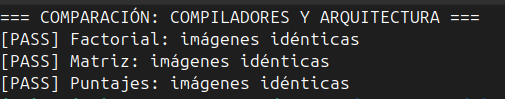
\includegraphics[width=0.9\textwidth]{img/04_comparacion.png}
    \caption{Comparación de imágenes de instrucciones
    entre Compiladores y Arquitectura.}
    \label{fig:integracion-arquitectura}
\end{figure}

\subsection{Ejercicio 1:
factorial}\label{81-ejercicio-1-factorial}

\subsubsection{Objetivo:} calcular el factorial de 5 con variables
locales, condicional y ciclo.
\subsubsection{Resultado esperado:}
\texttt{resultado = 120}. En el fuente,
\texttt{resultado} comienza en 1 e
\texttt{i} comienza en 2. En cada iteración se
multiplica el acumulador por \texttt{i} y se incrementa
\texttt{i}.
\subsubsection{Evidencia de compilación aportada:} 189 bundles, 7 saltos, 1
reescrito, archivo BAL de \textbf{3072 bytes}.

\subsubsection{Evolución matemática esperada, NO ejecución observada:}

\begin{longtable}[]{@{}rrr@{}}
\toprule\noalign{}
Paso & \texttt{i} procesado &
\texttt{resultado} \\
\midrule\noalign{}
\endhead
\bottomrule\noalign{}
\endlastfoot
Inicial & --- & 1 \\
1 & 2 & 2 \\
2 & 3 & 6 \\
3 & 4 & 24 \\
4 & 5 & 120 \\
\end{longtable}

\subsubsection{Validación de ejecución en la arquitectura VLIW}

El programa factorial fue ejecutado mediante
la infraestructura de simulación RTL utilizando
Icarus Verilog.

La prueba de integración finalizó satisfactoriamente,
confirmando la coincidencia de tres registros y
tres palabras de memoria con los valores esperados.

\begin{lstlisting}[caption={Validacion RTL del factorial}]
FACTORIAL: n=5, resultado esperado=120
[PASS] 3 registros y 3 palabras coinciden

x14 = 0x00000078

[PASS] Imagen ejecutada identica a la de Compiladores
\end{lstlisting}

El registro \texttt{x14} contiene el valor
hexadecimal \texttt{0x78}, equivalente a 120
en decimal.

Por tanto, la ejecución del factorial produjo
el resultado esperado y la validación RTL
finalizó satisfactoriamente.

\begin{figure}[H]
    \centering
    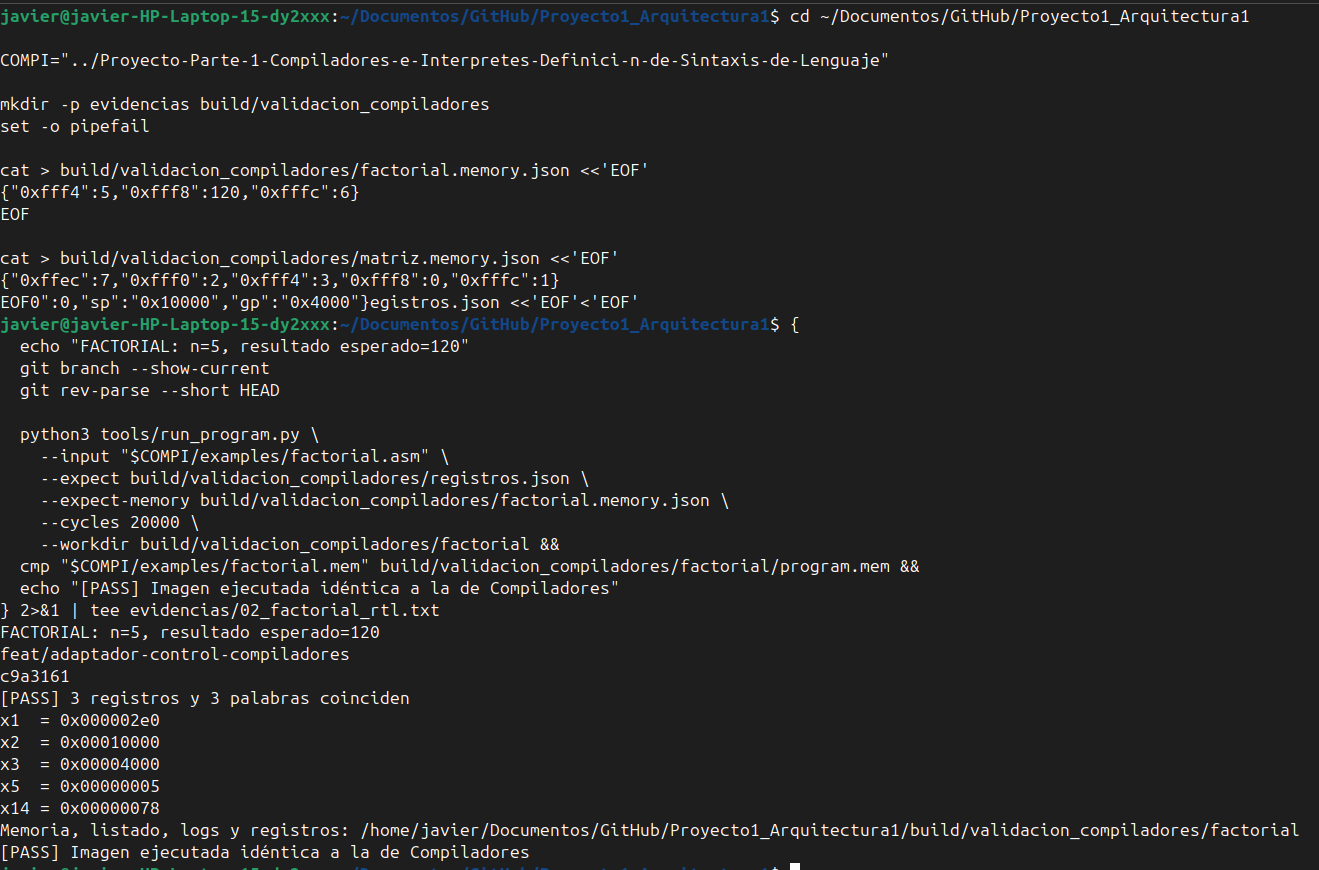
\includegraphics[width=\textwidth]{img/factorial_rtl.png}
    \caption{Evidencia de ejecución del factorial
    en la arquitectura VLIW mediante Icarus Verilog.}
    \label{fig:factorial-rtl}
\end{figure}

\subsubsection{Traza dinámica de ejecución}

La simulación permitió observar los cambios de la
variable \texttt{resultado}, almacenada en
la dirección \texttt{0xFFF8}.

Durante la ejecución, su valor evolucionó
de 1 a 2, 6, 24 y finalmente 120.

La repetición de la instrucción de almacenamiento
en la dirección \texttt{0x0A20} evidencia
las iteraciones del ciclo utilizado para
calcular el factorial.

\begin{figure}[H]
    \centering
    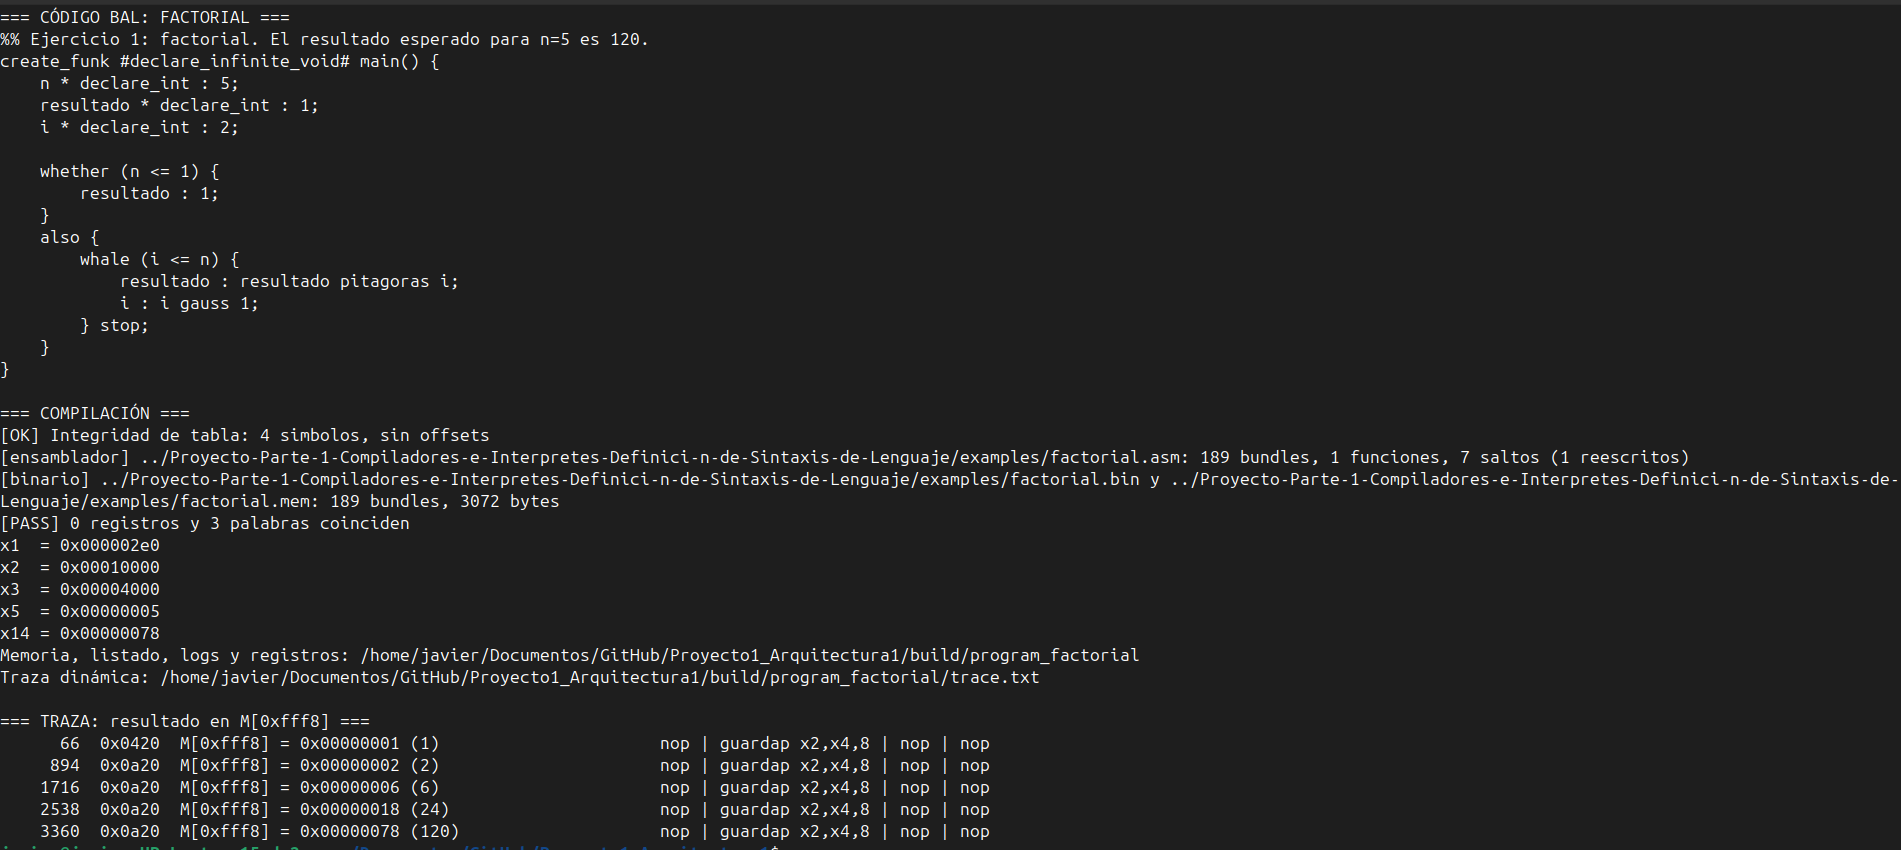
\includegraphics[width=\textwidth]{img/01_factorial.png}
    \caption{Traza dinámica del cálculo del factorial
    mediante la arquitectura VLIW.}
    \label{fig:traza-factorial}
\end{figure}

\subsection{Ejercicio 2: búsqueda en
matriz}\label{82-ejercicio-2-buxfasqueda-en-matriz}

\subsubsection{Objetivo:} buscar la primera aparición de 7 en
\texttt{[[4,7,1],[9,5,7]]} mediante dos ciclos
\texttt{whale}. El programa inicializa la posición a
\texttt{(-1,-1)} y actualiza el primer hallazgo.
\subsubsection{Resultado esperado:}
\texttt{(fila\_encontrada, columna\_encontrada) = (0, 1)}.

\subsubsection{Evidencia de compilación aportada:} 132 tokens, AST construido,
validación semántica, 7 símbolos, marco de 48 bytes, 291 bundles, 8
saltos resueltos, 2 reescritos, 2 vueltas de enlace, archivo BALB de
\textbf{4704 bytes}.
\subsubsection{Evolución conceptual esperada, NO ejecución observada:}

\begin{longtable}[]{@{}lrll@{}}
\toprule\noalign{}
Posición examinada & Valor & ¿Es primer 7? & Posición almacenada \\
\midrule\noalign{}
\endhead
\bottomrule\noalign{}
\endlastfoot
(0,0) & 4 & No & (-1,-1) \\
(0,1) & 7 & Sí & (0,1) \\
(0,2) & 1 & No & (0,1) \\
(1,0) & 9 & No & (0,1) \\
(1,1) & 5 & No & (0,1) \\
(1,2) & 7 & Ya hubo un hallazgo & (0,1) \\
\end{longtable}

\subsubsection{Validación de ejecución en la arquitectura VLIW}

El programa de búsqueda en matriz fue ejecutado
mediante la infraestructura de simulación RTL
utilizando Icarus Verilog.

La prueba verificó la coincidencia de tres
registros y cinco palabras de memoria
con los valores esperados.

\begin{lstlisting}[caption={Validacion RTL de la matriz}]
MATRIZ: posicion esperada = fila 0, columna 1
[PASS] 3 registros y 5 palabras coinciden

x5  = 0x00000002
x6  = 0x00000001

[PASS] Imagen ejecutada identica a la de Compiladores
\end{lstlisting}

La validación finalizó satisfactoriamente
y confirmó la coincidencia de los valores
verificados con los resultados de referencia.

El resultado esperado del algoritmo es
la posición $(0,1)$, correspondiente a
la primera aparición del valor buscado.

\begin{figure}[H]
    \centering
    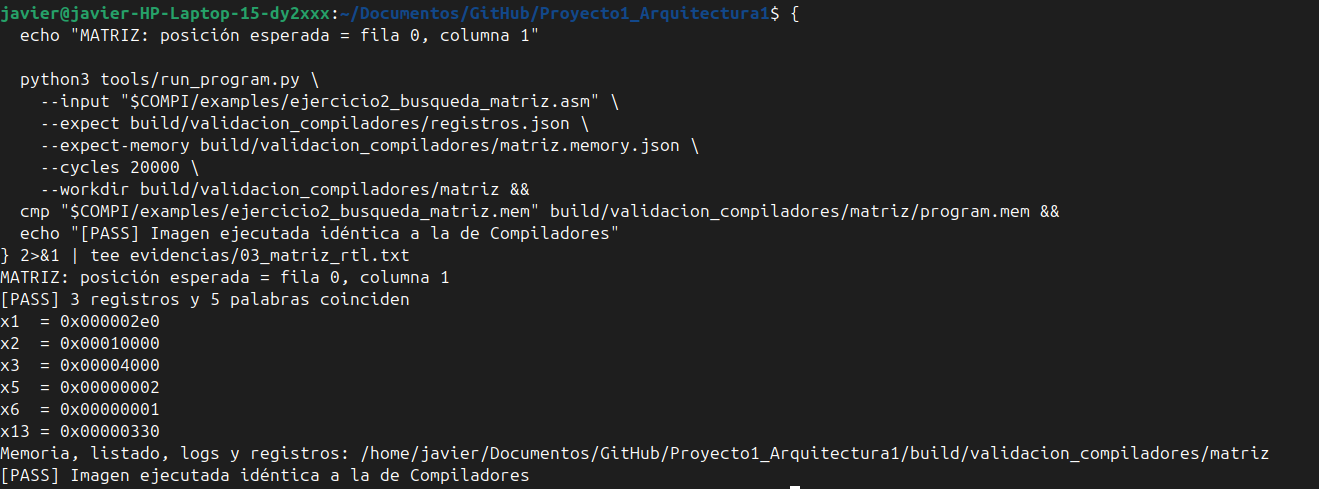
\includegraphics[width=\textwidth]{img/matriz_rtl.png}
    \caption{Evidencia de ejecución de la búsqueda en una matriz
    en la arquitectura VLIW mediante Icarus Verilog.}
    \label{fig:factorial-rtl}
\end{figure}

\subsubsection{Traza dinámica de ejecución}

La simulación permitió verificar los cambios de
las variables \texttt{fila\_encontrada} y
\texttt{columna\_encontrada}.

Inicialmente, ambas variables fueron almacenadas
con el valor -1.

Posteriormente, durante la búsqueda en la matriz,
sus valores cambiaron a 0 y 1, respectivamente,
confirmando que el programa identificó la primera
aparición del valor buscado en la posición (0,1).

\begin{figure}[H]
    \centering
    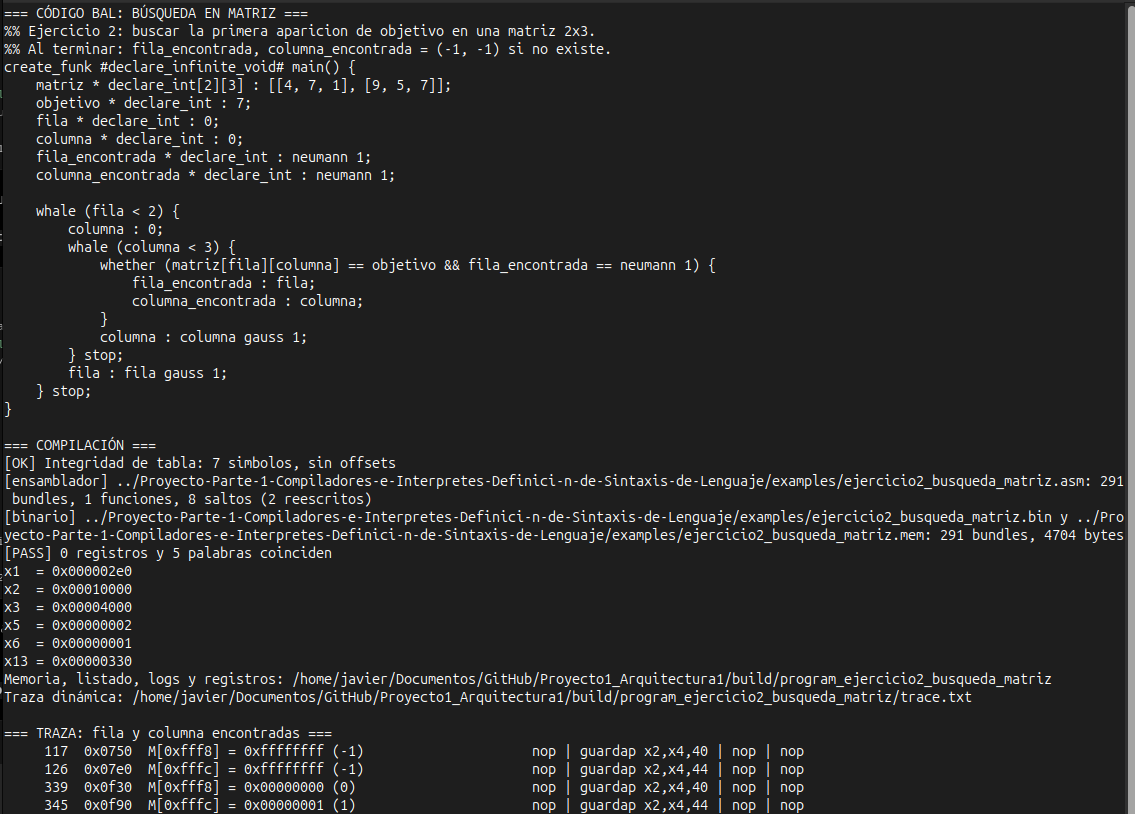
\includegraphics[width=\textwidth]{img/02_matriz.png}
    \caption{Traza dinámica de la búsqueda
    en una matriz bidimensional.}
    \label{fig:traza-matriz}
\end{figure}


\subsection{Ejercicio 3: funciones y puntajes}
\label{83-ejercicio-3-funciones-y-puntajes}

\subsubsection{Objetivo:} demostrar funciones
\texttt{sumar}, \texttt{puntaje} y
\texttt{acumular}, parámetros, retornos,
anidación de estructuras de control y
llamadas encadenadas.

\subsubsection{Resultado esperado:}
\texttt{resultado = 24},
\texttt{vacio = 0},
\texttt{combinado = 13} y
\texttt{total = 37}.
El programa utiliza llamadas a funciones
con parámetros, valores de retorno y ciclos
para realizar los cálculos.

\subsubsection{Evidencia de compilación aportada:}
190 tokens, 0 errores léxicos, AST construido,
validación semántica satisfactoria,
15 símbolos, 4 funciones, marco máximo
de 20 bytes, 801 bundles, 6 saltos
resueltos, 1 reescrito, 4 vueltas de
enlace y archivo BALB de
\textbf{12\,864 bytes}.

\subsubsection{Evolución conceptual esperada,
NO ejecución observada:}

\begin{longtable}[]{@{}llr@{}}
\toprule\noalign{}
Paso & Operación & Resultado \\
\midrule\noalign{}
\endhead
\bottomrule\noalign{}
\endlastfoot
1 & \texttt{acumular(5)} & 24 \\
2 & \texttt{acumular(0)} & 0 \\
3 & \texttt{acumular(3)} & 10 \\
4 & \texttt{sumar(1,2)} & 3 \\
5 & \texttt{sumar(10,3)} & 13 \\
6 & \texttt{sumar(24,13)} & 37 \\
\end{longtable}

La compilación del Ejercicio 3 finalizó
satisfactoriamente y generó los archivos
de ensamblador y código máquina VLIW.

\subsubsection{Validación de ejecución en la arquitectura VLIW}

El programa de funciones y puntajes fue ejecutado
mediante la infraestructura de simulación RTL
utilizando Icarus Verilog.

La prueba de integración finalizó satisfactoriamente,
confirmando la coincidencia de tres registros
y cuatro palabras de memoria.

\begin{lstlisting}[caption={Validacion RTL de funciones y puntajes}]
PUNTAJES: resultados esperados = 24, 0, 13 y 37
[PASS] 3 registros y 4 palabras coinciden

x4 = 0x00000025
x5 = 0x0000000d
x8 = 0x00000025
x9 = 0x0000000d

[PASS] Imagen ejecutada identica a la de Compiladores
\end{lstlisting}

Los valores hexadecimales
\texttt{0x25} y \texttt{0x0D}
corresponden a 37 y 13 en decimal,
respectivamente.

Adicionalmente, la prueba verificó
cuatro palabras de memoria contra
los resultados esperados.

La integración entre BALC y la arquitectura
VLIW fue validada satisfactoriamente
para este ejercicio.

\begin{figure}[H]
    \centering
    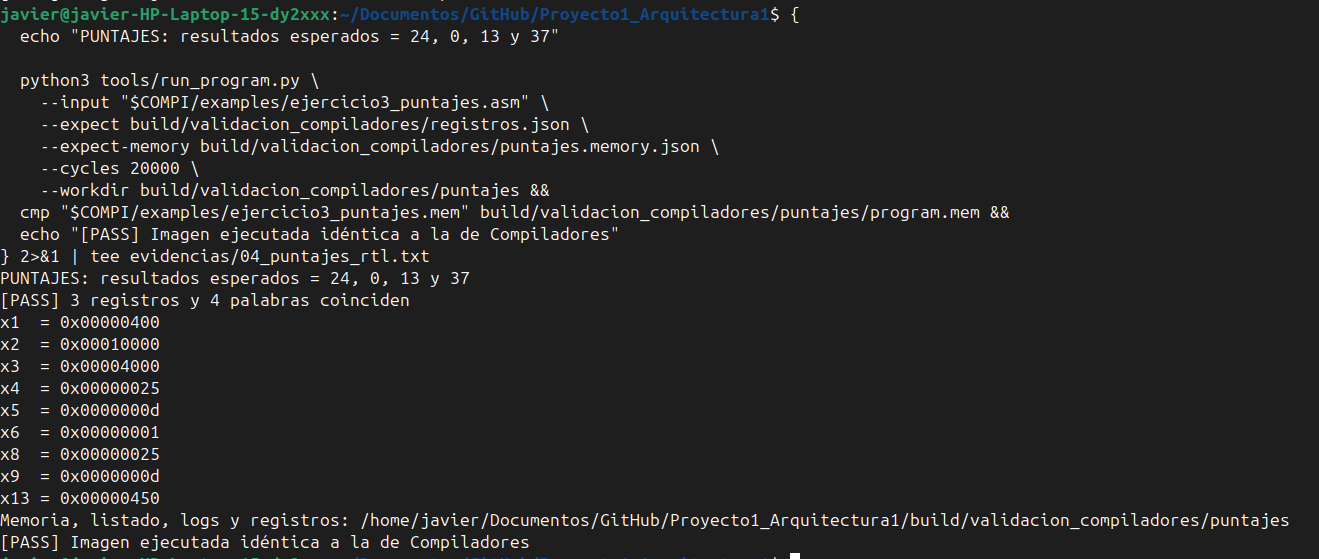
\includegraphics[width=\textwidth]{img/puntajes_RTL.png}
    \caption{Evidencia de ejecución de puntajes
    en la arquitectura VLIW mediante Icarus Verilog.}
    \label{fig:factorial-rtl}
\end{figure}

\subsubsection{Traza dinámica de ejecución}

La simulación permitió verificar las escrituras
en memoria correspondientes a las cuatro variables
de la función \texttt{main}.

Los valores registrados fueron:

\begin{itemize}
    \item \texttt{resultado = 24}.
    \item \texttt{vacio = 0}.
    \item \texttt{combinado = 13}.
    \item \texttt{total = 37}.
\end{itemize}

Estos resultados demuestran que las operaciones
con funciones, parámetros y valores de retorno
produjeron los resultados esperados.

\begin{figure}[H]
    \centering
    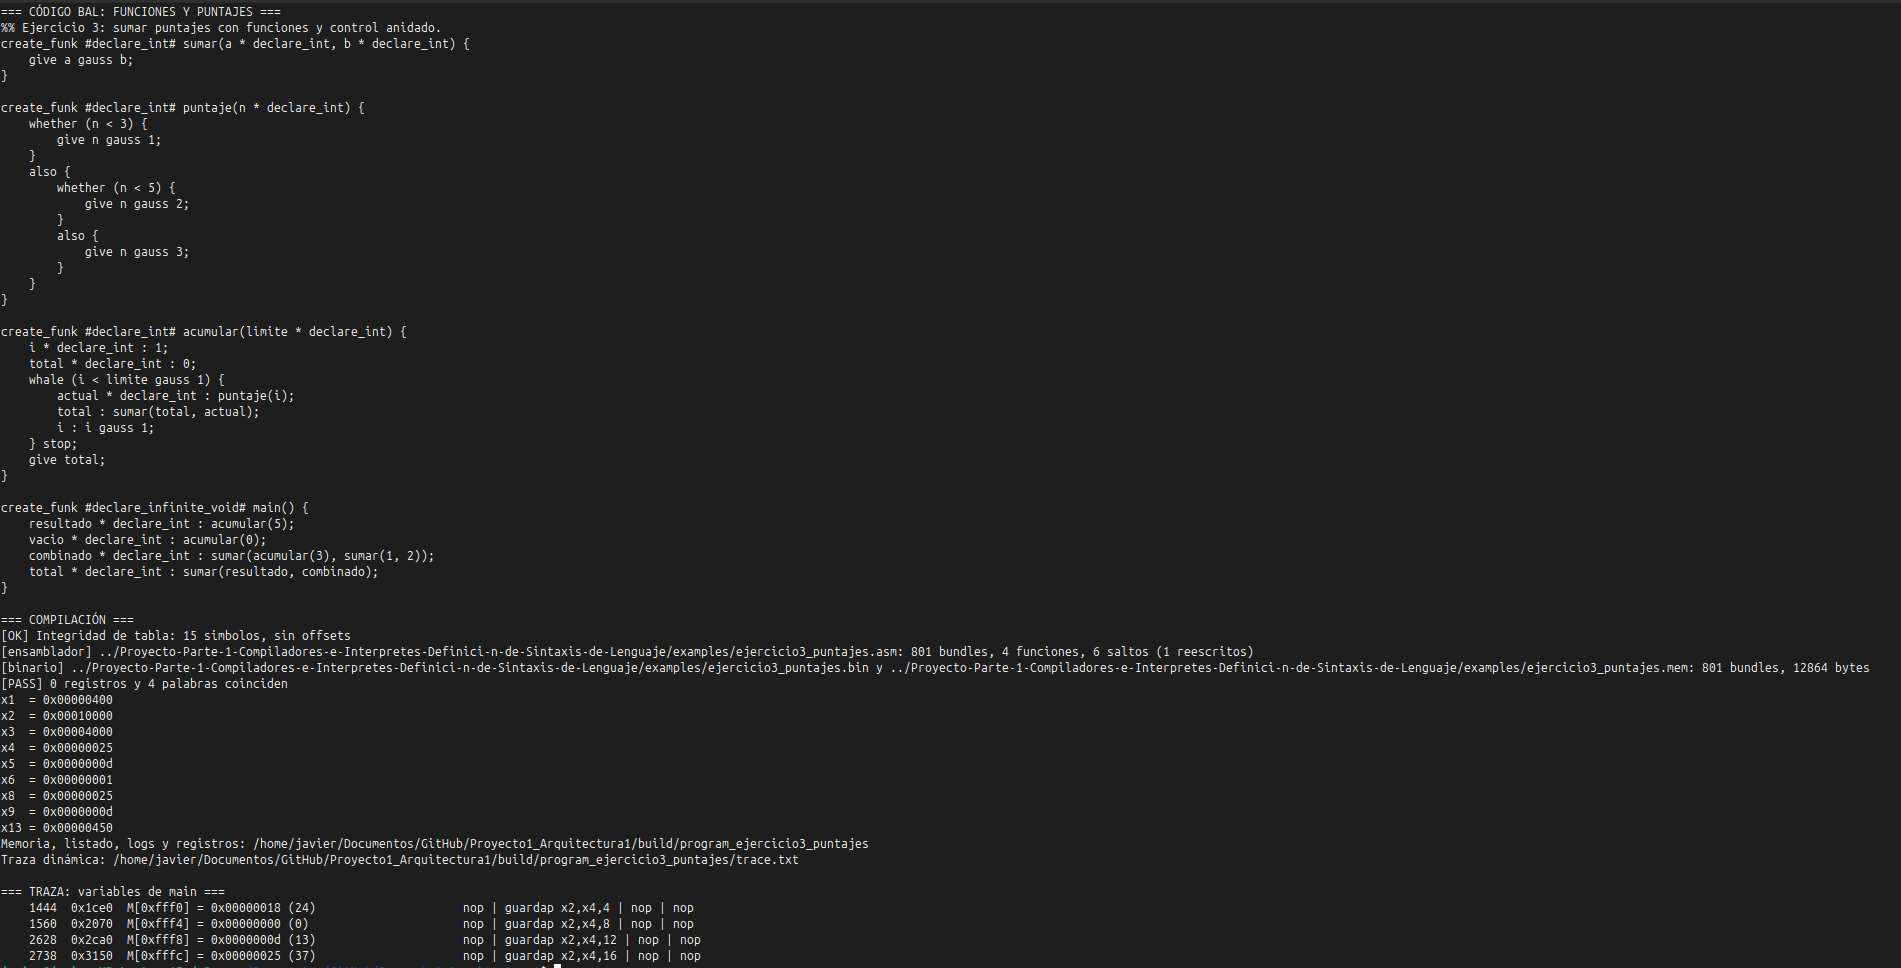
\includegraphics[width=\textwidth]{img/03_puntajes.png}
    \caption{Traza dinámica de las funciones
    y el cálculo de puntajes.}
    \label{fig:traza-puntajes}
\end{figure}


\section{Manejo de casos especiales}\label{9-manejo-de-casos-especiales--apartado-85}

\begin{longtable}[]{@{}p{0.25\linewidth}p{0.660\linewidth}@{}}
\toprule\noalign{}
Caso & Estrategia implementada y comprobación \\
\midrule\noalign{}
\endhead
\bottomrule\noalign{}
\endlastfoot
Condicional dentro de ciclo & AST anidado, generación de etiquetas y
saltos, pruebas de layout y saltos anidados. \\
Salto condicional lejano & Expansión a condición invertida seguida de
\texttt{sye}, con relayout hasta estabilización. \\
Funciones y retornos & Firmas registradas en primera pasada, parámetros
y \texttt{give} validados, llamada/enlace y
preservación de retorno. \\
Identificadores homónimos & Ámbitos de función/bloque y búsqueda desde
el ámbito actual hacia los externos. \\
Variable global frente a local & Almacenamiento
\texttt{gp} o marco \texttt{sp} con
offset concreto. \\
Índices de matrices & Número y tipo de índices; comprobación de rango si
la longitud y el índice son constantes. \\
Intento de modificar constante & Diagnóstico semántico incluso para
destino indexado. \\
Capturas \texttt{seek}/\texttt{seize}
& Diagnósticos semánticos y ámbitos propios; sin evidencia de runtime de
excepciones. \\
Importaciones & Registro semántico y resolución condicionada a callback;
no extrapolar a enlace multiarhivo completo. \\
Arreglos/listas dinámicos & Frontend y validaciones semánticas posibles;
no declarar soporte total del backend sin prueba. \\
\end{longtable}


\section{Pruebas y evidencias
reproducibles}\label{10-pruebas-y-evidencias-reproducibles}

\subsection{Pruebas automatizadas aportadas por el
equipo}\label{101-pruebas-automatizadas-aportadas-por-el-equipo}

\begin{xltabular}{\textwidth}{
    @{}
    >{\hsize=1.10\hsize\linewidth=\hsize\raggedright\arraybackslash}X
    >{\hsize=0.90\hsize\linewidth=\hsize\raggedright\arraybackslash}X
    @{}
}
\toprule
Comando & Resultado informado \\
\midrule
\endhead

\bottomrule
\endlastfoot

\path{make test-symbol-table} &
Prueba exitosa. \\

\addlinespace

\path{make test-semantic} &
OK: AST, no declarados, tipos y duplicados. \\

\addlinespace

\path{make test-semantic-functions} &
OK: argumentos, retornos y \texttt{main};
casos de error rechazados. \\

\addlinespace

\path{make test-semantic-matrix-cycle} &
OK: matrices, \texttt{cycle} y ámbitos. \\

\addlinespace

\path{make test-m-simbolos} &
OK: símbolos, memoria y errores. \\

\addlinespace

\path{make test-auditoria-semantica} &
OK: seis escenarios. \\

\addlinespace

\path{make test-referencias-integracion} &
OK: callbacks, offsets, etiquetas,
llamadas recursivas y rechazo sin layout. \\

\addlinespace

\path{make test-resolucion-saltos} &
OK: bundles, saltos anidados y largos,
funciones, arranque y arreglos. \\

\addlinespace

\path{make test-ejercicio2-matriz} &
OK: sintaxis, semántica, \texttt{-m},
binario y rechazo de índices. \\

\end{xltabular}

Los diagnósticos semánticos impresos en casos negativos son
esperados dentro de la prueba: esta tiene éxito cuando el
compilador rechaza la entrada inválida.

\subsection{Compilación detallada del Ejercicio
2}\label{102-compilaciuxf3n-detallada-del-ejercicio-2}

\begin{lstlisting}
[fase 1] lexico: 132 tokens, 0 errores
[fase 2] sintactico: AST construido
[fase 3] semantico: declaraciones, tipos, ambitos y llamadas validos
[fase 3] memoria: 1 funciones, marco maximo 48 bytes
[fase 4] ensamblador: arranque en 0x0000 llama a main; main en 0x0330
[fase 5] saltos: 8 resueltos, 2 reescritos; 2 vueltas de enlace; 291 bundles
[fase 6] binario: 291 bundles codificados y validados
[binario] ... .bin y .mem: 291 bundles, 4704 bytes
\end{lstlisting}

\textbf{Interpretación:} esto demuestra las etapas de compilación y
generación de los archivos. No demuestra que el procesador haya
ejecutado el binario.

\subsection{Evidencia mínima de código
máquina}\label{103-evidencia-muxednima-de-cuxf3digo-muxe1quina}

\begin{lstlisting}
Paquete 0138 -- PC=0x08a0
ensamblador: nop | nop | igualno x4,x0,96 | nop
hex (CRIPTO BRU LSU ALU): 00000000 82440060 00000000 00000000

Paquete 0264 -- PC=0x1080
ensamblador: nop | nop | sye x0,-1824 | nop
hex (CRIPTO BRU LSU ALU): 00000000 9600f8e0 00000000 00000000
\end{lstlisting}

\section{Uso, reproducción y
entrega}\label{12-uso-reproducciuxf3n-y-entrega}

\begin{lstlisting}[language=bash]
# Compilacion
make

# Ejercicios (ensamblador + binario + imagen de memoria)
./balc -v -s -m -p examples/factorial.bal
./balc -v -s -m -p examples/ejercicio2_busqueda_matriz.bal
./balc -v -s -m -p examples/ejercicio3_puntajes.bal

# Pruebas completas
make test

# Otras opciones
./balc -x -p examples/factorial.asm
\end{lstlisting}

\newpage

\section{Anexos técnicos de los tres
programas}\label{14-anexos-tuxe9cnicos-de-los-tres-programas}
Los ejercicios solicitados se pueden encontrar en las siguientes rutas dentro del repositorio:
\begin{itemize}
    \item Ejercicio 1 (Factorial): \path{examples/factorial.bal}
    \item Ejercicio 2 (Búsqueda en matriz): \path{examples/ejercicio2_busqueda_matriz.bal}
    \item Ejercicio 3 (Puntajes) : \path{examples/ejercicio3_puntajes.bal}
\end{itemize}

Debido a la extensión del .bal, el código ensamblador y de su
representación hexadecimal, se presentan en este
documento fragmentos representativos de los tres
ejercicios.

Los listados completos se incluyen como archivos
complementarios de la entrega, en los formatos
\texttt{.asm} y \texttt{.mem}, dentro del directorio
\texttt{examples/}.
\newpage
\subsection{Ejercicio 1}
\textbf{Fragmento de código fuente BAL:}

\begin{lstlisting}[caption={Ejercicio 1: ciclo del factorial}]
whale (i <= n) {
    resultado : resultado pitagoras i;
    i : i gauss 1;
} stop;
\end{lstlisting}

\textbf{Fragmento de ensamblador generado:}

\begin{lstlisting}[caption={Ejercicio 1: salto condicional VLIW}]
# PC = 0x0570
nop | nop | igualsi x4,x0,192 | nop
\end{lstlisting}

\textbf{Representación hexadecimal:}

\begin{lstlisting}[caption={Ejercicio 1: bundle hexadecimal}]
# PC = 0x0570
00000000822400c00000000000000000
\end{lstlisting}

\subsection{Ejercicio 2}
\textbf{Fragmento de código fuente BAL:}

\begin{lstlisting}[caption={Ejercicio 2: busqueda en matriz}]
whale (fila < 2) {
    columna : 0;

    whale (columna < 3) {
        whether (matriz[fila][columna] == objetivo
                 && fila_encontrada == neumann 1) {
            fila_encontrada : fila;
            columna_encontrada : columna;
        }

        columna : columna gauss 1;
    } stop;

    fila : fila gauss 1;
} stop;
\end{lstlisting}

\textbf{Fragmento de ensamblador generado:}

\begin{lstlisting}[caption={Ejercicio 2: resolucion de saltos}]
# PC = 0x08a0
nop | nop | igualno x4,x0,96 | nop

# PC = 0x08d0
nop | nop | sye x0,2256 | nop
\end{lstlisting}

\textbf{Representación hexadecimal:}

\begin{lstlisting}[caption={Ejercicio 2: bundles hexadecimales}]
# PC = 0x08a0
00000000824400600000000000000000

# PC = 0x08d0
00000000960008d00000000000000000
\end{lstlisting}

\subsection{Ejercicio 3}

\textbf{Fragmento de código fuente BAL:}

\begin{lstlisting}[caption={Ejercicio 3: funciones y puntajes}]
create_funk #declare_int# sumar(
    a * declare_int,
    b * declare_int
) {
    give a gauss b;
}

create_funk #declare_int# acumular(
    limite * declare_int
) {
    i * declare_int : 1;
    total * declare_int : 0;

    whale (i < limite gauss 1) {
        actual * declare_int : puntaje(i);
        total : sumar(total, actual);
        i : i gauss 1;
    } stop;

    give total;
}
\end{lstlisting}
\newpage
\textbf{Fragmento de ensamblador generado:}

\begin{lstlisting}[caption={Ejercicio 3: operaciones y saltos}]
# Funcion sumar, PC = 0x0570
suma x4,x4,x5 | nop | nop | nop

# Funcion acumular, PC = 0x0ea0
nop | nop | igualno x4,x0,96 | nop

# Funcion acumular, PC = 0x0ed0
nop | nop | sye x0,2400 | nop
\end{lstlisting}

\textbf{Representación hexadecimal:}

\begin{lstlisting}[caption={Ejercicio 3: bundles hexadecimales}]
# PC = 0x0570
000000000000000000000000d5042140

# PC = 0x0ea0
00000000824400600000000000000000

# PC = 0x0ed0
00000000960009600000000000000000
\end{lstlisting}
\end{document}
